% TODOS
% Hinweise Grundlagen anpassen
% Bisschen konkreter


% Der Mensch kann ziemlich gut generalisieren
% Medical AI kann das lernen

% Wie lernen Kinder -> Wie viele Beispiele bruachen Kinder?
% Wie viele brauchen Maschinen

\section{Motivation} % p 2.5
    Clinical diagnostics and research has been improved dramatically with emergence of volumetric imaging such as \ac{CT} and \ac{MRI} technology which enables visualizing body parts and organs.
    In recent years, \ac{CT} examinations have increased substantially in many countries \citep{westmark2023increasing, masjedi2020european, martella2023diagnostic}. The importance of \ac{MRI} scans, which offer better soft-tissue contrast without exposing radiation to the patient examined, has likewise increased reaching above 200 scans per 1000 people in some countries in 2020 \citep{martella2023diagnostic}.
    % TODO Are there some papers that have evidence for benefit of methods?

    Volumetric imaging offers the benefit of capturing the organ of interest in its \ac{3D} space. However, visualizing the \ac{3D} volume is performed on \ac{2D} screens where in case of \ac{CT} and \ac{MRI}
    % a suitable form of \ac{3D} projection for the densly acquired volume has to be found or
    individual view planes / imaging slices have to be selected for examination. Automated processing is needed
    % in the first case
    for the visualization
    % itself and in the latter case automated processing
    and can support clinicians navigating the \ac{3D} volume, help classifying organ boundaries, measuring tumour sizes and highlight organ deformations, all of which is complicated to perform manually when navigating a \ac{3D} volume in \ac{2D} space.

    Deep learning with its basic principles invented in the last century, has become a de-facto standard now for automated processing in versatile fields such as for processing text, images, audio, video, analogous signals, biological processes or physical agent simulations
    \citep{%
        ouyang2022training, %text
        kirillov2023segment, %images
        birtchnell2018listening,%audio
        huang2020movienet,%video
        sahoo2020machine,%analogous signals (ecg)
        jumper2021highly,%biological processes
        makoviychuk2021isaac,%physical interaction ,%agent simulations
    }
    and has created a significant technology push throughout all of the mentioned areas of application.
    Of course, this holds true for (volumetric) medical image analysis as well, where formerly hand-crafted method design is now combined or even entirely replaced with data-driven, learning-based methods \citep{hosny2018artificial, rajpurkar2022ai}.

    Deep learning as a special concept of artificial learning, was sought to mimick the neuronal activity in brain tissue. It has been found that higher-level concepts of human learning such as reasoning about generalization applies to deep learning in similar ways \citep{jakel2008generalization}. Shifting our view to the main topic of this thesis a question is raised to the reader:

    \begin{quote}
        \centering \Large
        What is \emph{generalization?}
        % $\vdots$
    \end{quote}

    \begin{figure}
        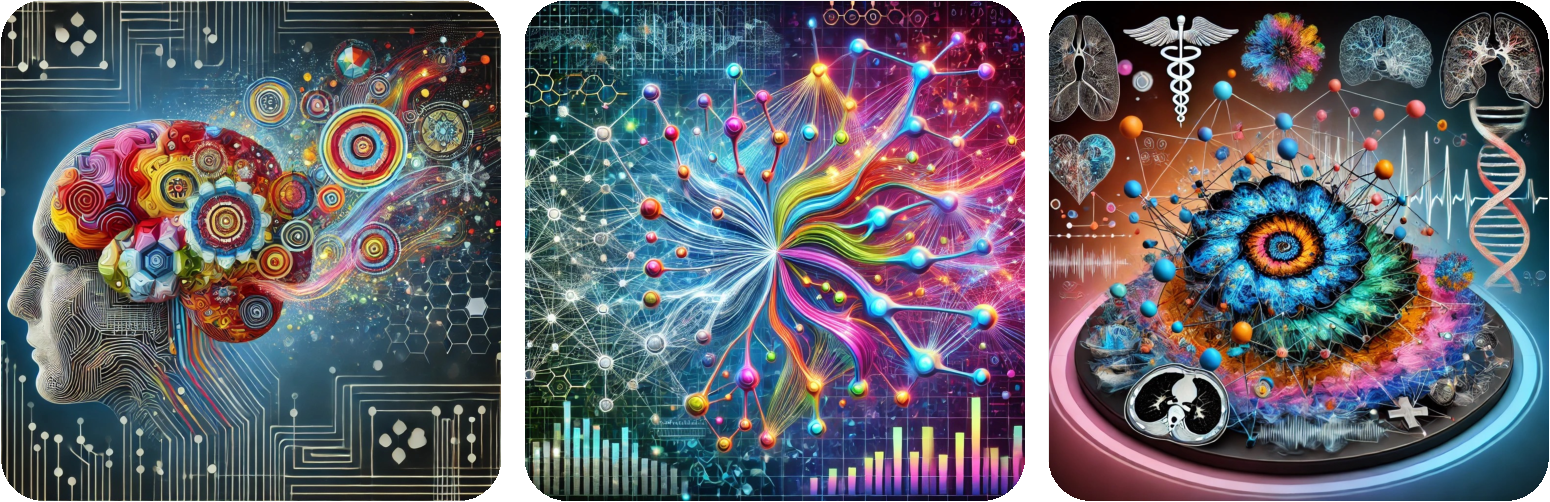
\includegraphics[width=\textwidth]{sections/01_introduction/figures/synthesized_generalization.pdf}
        \caption{Visualizations of a state-of-the-art text-to-image generator DALL$\cdot$E 3 \citep{betker2023improving} when prompted to \textquote{visualize generalization} (left), to \textquote{visualize generalization in deep learning} (middle) and to \textquote{visualize generalization in deep learning for volumetric medical images} (right).}
        \label{fig:synthesized_generalization}
    \end{figure}

    % This question will serve us as starting point to motivate the main aspects of this thesis.
    As a help for brainstorming, a deep learning-based text-to-image generator \citep{betker2023improving} was prompted to visualize \textquote{generalization}, \textquote{generalization in deep learning} and \textquote{generalization for volumetric medical images} (see \figref{fig:synthesized_generalization}).
    % In the following lines, the above raised question is answered using the generative output of \figref{fig:synthesized_generalization}.

    \textquote{Generalization} (\figref{fig:synthesized_generalization}, left) was depicted as a human brain related topic, showing abstract organic shapes emerging from the central skull boundary.
    % as well as regular wire-like structures at the top and bottom of the image.
    The initial definition of generalization is indeed brain related and was described for fear learning, where two sub-mechanisms of conditioned learning --- generalization and specialization --- were discovered \citep{banich2011generalization}. % TODO primary source needed
    In fear learning, initially an instance-based generalization\footnote{Opposed to the presented finding, in deep learning, specialization is considered to be formed instance-based} occurs that maps a novel fear to an environment \citep{banich2011generalization}.
    % Later, this generalization is specialized and mapped to specific environmental stimuli leading to the learning of discriminative aspects \citep{banich2011generalization}.

    The visualization for \textquote{generalization in deep learning} is showing such a network of nodes with connecting lines inbetween these nodes and lead us to a different \emph{level} in which learning processes can be analyzed.
    Learning (of generalization) on the cell level, is assumed to work as the change of neuron (nodal) connection-strength through synaptic plasticity \citep{do1949organization, martin2000synaptic}.
    % Researching the biological learning process requires different levels of abstractions, such as contextual behavioural and psychological studies, understanding brain macro activity, as well as cell level experiments.

    The investigation of principal conditioned learning mechanisms in the last century revealed, that learning is context based and described as the association of an experienced stimulus (input) to an expectation (output)
    % e.g. a dog that awaits food after hearing the sound of a bell
    \citep{pavlov1928conditioned, pavlov2010conditioned, banich2011generalization}. This implies that learning must not only be analyzed on different levels but also in varying contexts and \emph{areas}.

    As synthesized in \figref{fig:synthesized_generalization} (right),
    this thesis will explore various different areas of volumetric medical imaging, namely different organs, different types of tasks such as segmentation and shape reconstruction as well as different imaging modalities.

    In deep learning, the ability of models to generalize is like in biological learning a desirable aspect.
    The mechanisms of artificial generalization are an active area of research but have not been understood or even solved entirely yet.
    This is also due to the fact that deep learning models are considered a blackbox model and forming an understanding of the internal reasoning of the models is hard, if not impossible.
    A trained deep learning model should still work if the specific anatomy in question is visible regardless of the individual image properties of the scanner used to acquire the image to enable a reliable analysis but it was often shown that even current methods for generalizing learning struggle under imaging domain shifts \citep{ouyang2022causality}.

    % This thesis will likewise investigate the differnt levels of data acquisition, data presentation, training and inference strategies, as well as model kernel level design to find elements necessary for generalization.
    The above mentioned findings lead us to the final research question of this thesis:

    \begin{quote}
        \centering \Large
        In which areas and on which levels can

        \noindent \emph{Generalization in Deep Learning Methods for Volumetric Medical Image Analysis}

        \noindent be enabled and improved?
        % $\vdots$
    \end{quote}

    % It is not enough to only look at the biological cells or their deep learning neuron equivalents, but at tasks' contexts, the encountered stimuli (data samples) as well as the learning processes.
    % Due to these reasons, this thesis investigates the elements to enable and optimize deep learning generalization for volumetric medical image analysis while looking wholistically along the processes of data acquisition, data presentation, model design as well as model training and inference strategies.


    % A general concept may thus only be formed if \emph{all} possible stimuli had been encountered. This is plain impossible for real learning and deep learning as well.

    % When training deep learning models, over-specialization is an often experienced challenge which is more technically referred to as overfitting and undesirable as it limits the performance of trained models for unseen data points \citep{xx}.

    % in human learning, generalization enables the transfer of an experienced stimulus or input to a broader context \citep{xx}.

    % , whereas specialization narrows generalized concepts down to more individual cases \citep{xx}.
    % Both steps were first described for fear-learning \citep{xx}.
    % % TODO explain concept of the study.

    % Over-generalization can lead to anxiety disorders in this regard \citep{xx}, whereas over-specialization can lead to missclassify dangerous situations. These mechanisms could be tracked down to individual parts of the brain: The amygdala is responsible for generalization whereas specialization occurs in the prefrontal cortex and the hippocampus \citep{banich2011generalization}.

    % In many technical applications the comparison with survival situations in biological learning may seem drastical, but in medical deep learning this scenario is not too far away, where misinterpretation during automated processing can results in misdiagnosis and potentially impact patients recovery or in the most extreme situations survival.

    % General deep learing findings
    % DL boosted and is boosting performance and outcome in versatile applications. This spans large areas
    % text processing
    % image processing
    % audio processings
    % video processing for robotics
    % robotics itself, sensors actuators
    % analog signals
    % biological processes
    % explorative agent simulations
    % physical applications
    % computer graphics

    % before: spezialized algorithms, frameworks
    % now: models can be used interchangebly with adjustmens to fit the target task at hand.

    % the idea is learning itself - defined as.

    % universal function approximators, but highly dependent on the data as the model itself isnt worth anything before it has been adjusted (trained).
    % AGI - is of recent discussion where some models reach impressive results.

    % this brings us to the term generalization ...
    % Generalization
    % Wholistic models
    % what is needed for learning in the first place?

    % enough data can fit everything

    % still  problems, halluzinations, intransparency,

    % generalization can be tackeled at different stages of the medical image processing pipeline
    % model optimizing?
    % data curation is necessary?

    % can we do sth at training, model application?

    % Medical deep learing findings
    % as well as medical applications and processing of spezialized sensor data such as volumetric data as MRI CT.
    % especially for medical imaging where outcomes can have real world implications on fragile patients.
    % and can also be applied in the medical domain (SAM)

    % advent of deep learning in medical imaging

    % Definition of generalization


    \section{Objectives} % p 1.5
        In this thesis different areas and levels in which generalization can be enabled are explored. The different areas and levels are laid out in the following paragraphs.

        \paragraph{Areas of Exploration}
            % Given the relevance of volumetric medical imaging for several body parts and disease diagnosis, model generalization approaches should not only be developed for one medical task but ideally provide benefit for many different analysis tasks and be task-agnostic.
            This thesis will thus cover volumetric analysis tasks throughout several body parts and organs. The examined tasks comprise the following scenarios:

            Volumetric imaging of the heart has been proven to successfully to asses heart function e.g. via its time-varying end-sytole and end-diastole ventricular volumes
            \citep{pattynama1994evaluation}. % bernard2018deep %DL method
            Furthermore, assessing the cardiac chambers' shapes can yield valuable information for future risk prediction
            \citep{ly2022interpretable}. %DL method
            % In cardiac tasks the heart movement is of particular interest.
            Volumetric brain imaging can be utilized to detect brain lesions, tumours, other pathologies
            \citep{
                hering2024improving, %lesions %DL method
                uzunova2019unsupervised, %tumours and other %DL method
            }
            and follow-up scans enable the monitoring of tissue changes providing valuable information for treatment planning or evaluation
            \citep{baheti2021brain}. %DL method
            Abdominal body scans can yield valuable insight into the existence of cancerous tissue, pancreatitis, liver infection and spleen abnormalities (non-exhaustive list).
            \citep{caraiani2020indications}.
            % TODO improve this enumeration with more systematic cases
            Besides soft-tissues, volumetric imaging enables the detection and classification of bone fractures and other malformations \citep{kuo2022artificial}.
            The deep learning based analysis of the mentioned body parts imposes all their own different challenges, but model generalization methods should nevertheless be as agnostic as possible to be versatile. All developed methods of this thesis will be evaluated for various tasks and body areas or at least possibilites and limitations of the methods regarding other tasks are discussed.

            A further area of exploration covers the differrent scanners used for acquisition such as CT or MRI scanners. Both device methods differ subsantially in their physical priciple of acquisition and thus resulting images inherit vastly different tissue contrast properties which can be utilized according to the diagnostic questions at hand.
            When analysing these images with one deep learning model, the resulting image modality gap imposes a challenge. While deep learning methods can achieve outstanding results in the training domain, prediction quality can significantly be reduced when the learnt models are applied to images of a different scanner even within one modality \citep{pooch2020can}.
            % So generalization methods of this thesis will also explicitly cover scanner-induced domain shifts.

            The deep learning process itself has different areas to explore.
            The quality of automated assessment does not only depend on the model capabilities and configuration but also on the data that is fed to the model and the strategy that is used for model training given that data \citep{soviany2022curriculum}.
            Enabling generalization in any of these areas can reinforce the overall generalization and improve the final outcome which is investigated throughout this thesis. The following chapters will thus cover the areas of data acquisition, data aggregation, sample weighting, model design and the strategies to train the desinged models given the available data.

        \paragraph{Levels of Exploration}
            Perpendicular to the mentioned different areas, the generalization methods will be analyzed on different levels.

            The meta structure of this thesis is constructed out of two different levels: On the one hand, the clinical level outcome is presented and the gained improvements that generalization enables for clinicians and patients are discussed.
            On the other hand, improvements on the technical level are discussed.
            This clinical and technical level meta structure is also reflected by the organization of the thesis presented in the next section \secref{sec:organization}.

            On the technical level itself, progress towards generalizing methods is made in a similar fashion by optimizing on higher or lower modelling levels.
            On higher levels, the modelling of wholistic processes is optimized. On lower levels, individual parts of the training and inference pipeline such as modifications of the training loss function for curriculum learning are presented even down to individual parameter/kernel-level changes of the model that benefit generalization.

            % Looking at the data fed to the model, augmentation schemes on the image intensity-level are developed.

        \section{Organization and Contributions}  % p 3.5
            \label{sec:organization}
            The thesis is divided into three major parts:
            Foundations are laid in Chapter \ref{chap:background} \nameref{chap:background}, which is itself divided into clinical and methodological deep learning background.
            The following four chapters \ref{chap:acquisitionfocus} to  \ref{chap:dgtta} explain the developed generalizing methods in medical deep learning for volumetric images. Each of these four chaptes is itself divided into a self-contained introduction, description of the methodology, the experiment configuration and results as well as a discussion and conclusion for the method. % TODO check the individual structure
            \figref{fig:draft} highlights the major aspects of the four chapters which are explained in more detail now.

            \begin{figure}
                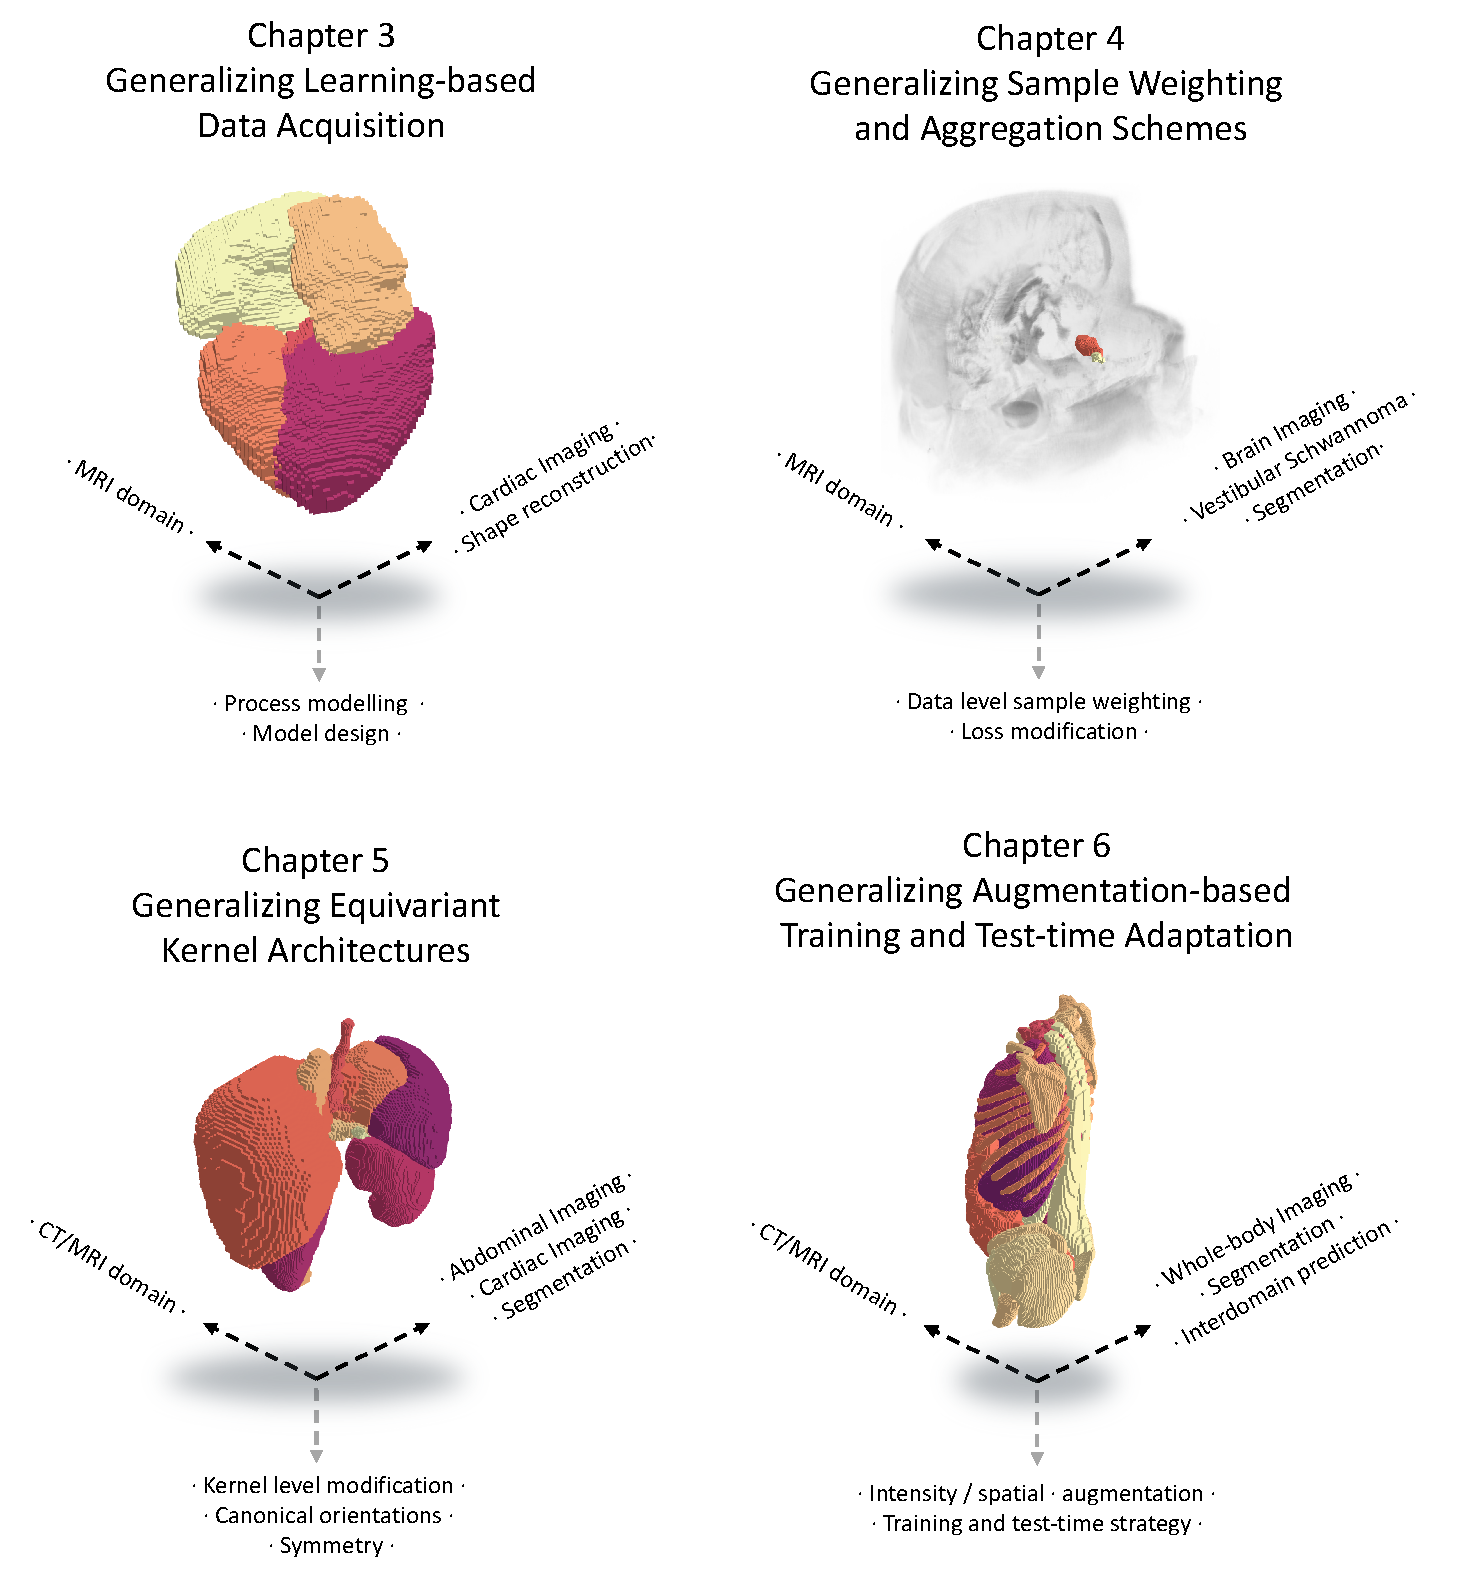
\includegraphics[width=\textwidth]{sections/01_introduction/figures/draft_areas_levels.pdf}
                \caption{Thesis organization: Four main chapters of this thesis will explore possible different areas and different levels for generalization. Different areas of exploration are described in the horizontal 3D plane. The levels of exploration are visualized perpendicular to the areas on the vertical axis of each chapter sub-figure.}
                \label{fig:draft}
            \end{figure}

            \begin{itemize}
                \item
                    In Chapter \ref{chap:acquisitionfocus} a wholistic view on the  high-level deep learning process is used to derive a concept for optimized data acquisition. Given a cardiac shape reconstruction task, the data acquisition process and the shape reconstruction model are jointly modelled and optimized to find generalizing MRI view planes describing the overall heart shape best. The ideas and methods were published in:

                    \vspace{1em}
                    \noindent\fullcite{weihsbach2023acquisitionfocus}

                    \vspace{1em}
                    \noindent\fullcite{weihsbach2024acquisitionfocus}

                \item
                    Chapter \ref{chap:dgtta} explains concepts to enable generalization for different imaging domains shifting view to the training and inference (application) phase of the model. Here, data augmentation is used to train models with generalizing capabilities to optimally segment various organs and bone structures given a large CT base dataset. The generalizing models are further optimized on individual MR images to optimize their performance when segmenting the same anatomical structures given very different image intensity distributions compared to the training domain. The method was published as a preprint in:

                    \vspace{1em}
                    \noindent\fullcite{weihsbach2023dg}

                \item
                    In Chapter \ref{chap:deepstaple} data aggregation and curriculum learning enable generalization on the data level. Applied to the task of vestibular schwanomma tumour and cochlea segmentation for differently weighted MR images, the method is developed to weight individual samples during the training phase of the model. This leads to the learning of a generalized shape representation given noisy, probably imperfect input labels derived by image registration. The method was published in:

                    \vspace{1em}
                    \noindent\fullcite{weihsbach2022deepstaple}

                \item
                    Moving to a lower level of detail, in Chapter \ref{chap:xedgeconv} modifications of the model kernels are explained that enable to learn generalized representations of organs to be segmented for differently oriented image volumes. This is especially interesting for the MRI domain, where image volumes can be acquired with arbitrary orientation.
                    The task-agnostic capabilities of the method were shown for an abdominal organ segmentation scenario as well as a cardiac chamber segmentation scenario.
                    The method was published in:

                    \vspace{1em}
                    \noindent\fullcite{weihsbach2022xedgeconv}


            \end{itemize}

            In the last chapter of this thesis \ref{chap:summary} \nameref{chap:summary} all of the findings are summarized again two-fold: The clinical impact of the mentioned contributions is evaluated with respect to the clinical benefit.
            Furthermore, technical improvements are discussed, not only yielding insight for deep learning in volumetric medical imaging but also for other fields of research.
